\section{制取蒸馏水}\label{sec:xssy-sy2}

\begin{shiyanmudi}
    1. 学习仪器装配的操作; 2. 学习蒸馏的操作。
\end{shiyanmudi}

\begin{shiyanyongpin}
    圆底烧瓶、导管、橡皮管、单孔橡皮塞、胶头滴管、试管、烧杯、酒精灯、铁架台(带铁圈和铁夹)、石棉网。

    高锰酸钾溶液。
\end{shiyanyongpin}

\begin{shiyanbuzhou}

    \begin{wrapfigure}[16]{r}{7cm}
        \centering
        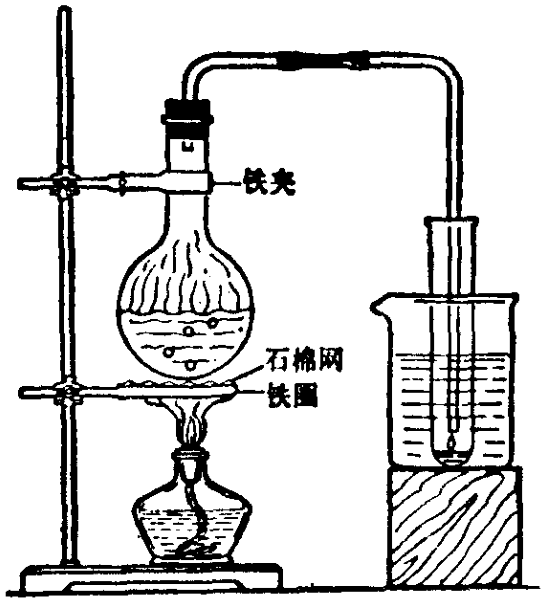
\includegraphics[width=6cm]{../pic/czhx1-xssy-17}
        \caption{制取蒸馏水的装置}\label{fig:xssy-17}
    \end{wrapfigure}

    1. 按化学实验基本操作五中仪器装配的要求,把烧瓶和导管连接好,并检查气密性。
    在烧瓶里倒入半瓶热水,用滴管取少量高锰酸钾溶液(观察它的颜色),
    把这种溶液滴入烧瓶里几滴,观察烧瓶里溶液的颜色。

    2. 按图 \ref{fig:xssy-17} 安装好仪器(注意酒精灯、铁圈和铁夹放置的位置)。
    烧杯中放入用来冷凝水蒸气的冷水。导管的末端应该跟试管底相距 2—3 厘米。
    为什么之必须保持这一段距离?

    3. 装置全部连接好以后,用酒精灯加热。加热的时候,注意不要使烧瓶里的液体沸腾得太厉害。
    如果沸腾得太厉害,液体就会直接通过导管流到试管里去(可以加几片碎瓷片,以防暴沸)。

    4. 观察蒸馏水的生成。用开始收集到的 2—3 毫升蒸馏水洗涤试管壁,倒掉。
    再用该试管收集 2—3 毫升蒸馏水,然后把导管从试管中取出,停止加热,取出试管。

    观察制得的蒸馏水的颜色,并与烧瓶里的液体颜色作比较。
\end{shiyanbuzhou}

\begin{wentihetaolun}

    1. 说出制得的蒸馏水的颜色,起初滴加的高锰酸钾最后残留在哪里?由此说明蒸馏的作用。

    2. 分别说出实验中使用的石棉网、铁夹和铁圈的作用。

\end{wentihetaolun}

